\documentclass{article}

\usepackage[margin=1in]{geometry}
\usepackage{amsmath,amssymb}
\usepackage{multicol}
\usepackage{float}
\usepackage{adjustbox}
\usepackage[spanish]{babel}
\usepackage[utf8]{inputenc}

\usepackage{graphicx}
\graphicspath{ {/Users/imagesLatex/} }

\begin{document}

\noindent
\begin{tabular*}{\textwidth}{l @{\extracolsep{\fill}} r @{\extracolsep{4pt}} l}
\text{} & \text{DEPARTAMENTO DE CIENCIA DE LA COMPUTACI\'ON}\\
\end{tabular*}\\
\rule[2ex]{\textwidth}{0.5pt}
\text{Base de Datos - IIC2413}\\
\text{Nombre Alumnos: Tanya Garrido - Rodrigo Zapata S.}\\
\text{Profesor: J. Reutter}\\
\text{Fecha: } \today\\
\rule[2ex]{\textwidth}{0.5pt}
\begin{center}
\Large\textbf{Tarea 1}\\
\end{center}

\noindent
\textbf{Parte 1: Modelaci\'on}

Primero se realiza un Diagrama Entidad/Relaci\'on del problema propuesto.
$ \\ $

\begin{center}
	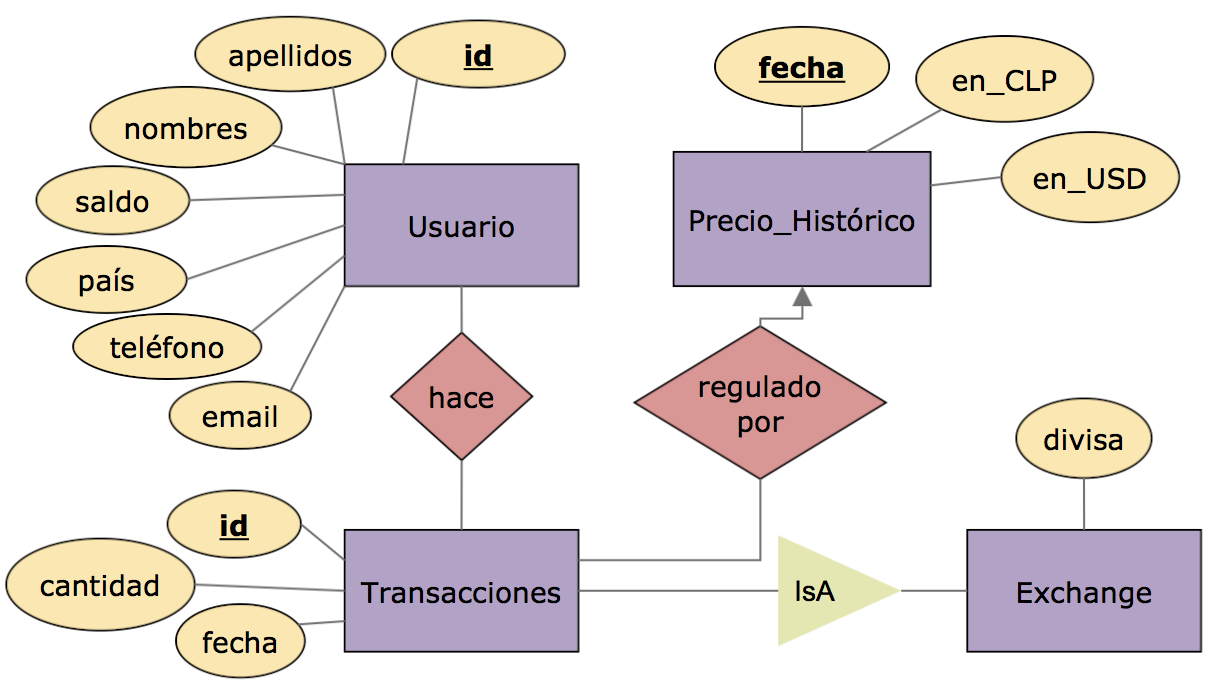
\includegraphics[width=0.6\textwidth]{Diagrama_ER.png}
\end{center}


Acontinuaci\'on se detallan las tablas creadas y sus respectivos atributos. El nombre del atributo se resaltar\'a con negrita y si el atributo es una llave, se resaltar\'a con un subrayado.

$ \\ $
\textbf{Usuarios}
\begin{itemize}
	\setlength{\itemindent}{.5in}
	\item{\underline{\textbf{id}} integer}
	\item{\textbf{nombres} varchar(30)}
	\item{\textbf{apellidos} varchar(30)}
	\item{\textbf{genero} varchar(30)}
	\item{\textbf{telefono} integer}
	\item{\textbf{mail} varchar(30)}
	\item{\textbf{pais} varchar(20)}
	\item{\textbf{saldo} float: cuantos zorzales posee la persona}
\end{itemize}

$ \\ $
\textbf{Transacciones}
\begin{itemize}
	\setlength{\itemindent}{.5in}
	\item{\textbf{rec\_id} integer: id de persona quien recibe el dinero}
	\item{\textbf{manda\_id} integer: id de quien transfiere dinero}
	\item{\underline{\textbf{id\_trans}} integer: id de la transacci\'on}
	\item{\textbf{fecha} varchar(20)}
	\item{\textbf{cantidad} float: cantidad de zorzales transferidos}
\end{itemize}

$ \\ $
\textbf{PreciosHistoricos}
\begin{itemize}
	\setlength{\itemindent}{.5in}
	\item{\textbf{\underline{fecha}} varchar(20)}
	\item{\textbf{z\_en\_usd} float: a cuantos dolares corresponde un zorzal}
	\item{\textbf{z\_en\_clp} float: a cuantos pesos chilenos corresponde un zorzal}
\end{itemize}
	
$ \\ $
\textbf{Exchange}
\begin{itemize}
	\setlength{\itemindent}{.5in}
	\item{\textbf{\underline{id}} integer}
	\item{\textbf{rec\_id} integer}
	\item{\textbf{manda\_id} integer}
	\item{\textbf{fecha} varchar(20)}
	\item{\textbf{cant\_transf} float}
	\item{\textbf{divisa} varchar(3): con que moneda paga quien transfiere, USD o CLP}
\end{itemize}

$ \\ $
Luego se detallan las independencias funcionales de los atributos:

\begin{itemize}
	\item{\textbf{En Usuarios:} id $ \rightarrow $ nombre, pais, mail, telefono, saldo}
	\item{\textbf{En Transacciones:} id $ \rightarrow $ rec\_id, manda\_id, fecha, cantidad}
	\item{\textbf{En Precios\_Hist\'oricos:} fecha $ \rightarrow $ en\_USD, en\_CHP}
	\item{\textbf{En Exchange:} id $ \rightarrow $ rec\_id, manda\_id, fecha, cantidad, divisa}
\end{itemize}

$ \\ $
Es posible notar que el esquema esta en BCNF, ya que para todo atributo $ X,Y $ tal que $ X \rightarrow Y $, entonces $ X $ es llave.

$ \\ $
Es posible notar tambi\'en que el esquema actual es igual al propuesto anteriormente, agregando simplemente los atributos $ genero $ y $ apellidos $ a la tabla Usuarios.




\end{document}